\section{Background and Motivation}
\label{sec:background_and_motivation}

We have been compelled by the idea to make the Zeroconf protocols available to web applications.
For example, consider the scenario of a group of people, each with their own device, collaborating on a Google Doc document.
Every keystroke in this document will need to be sent to a Google web server and then be ``pushed'' too all other group members.
Depending on geological location, this pattern of communication can impose roundtrips around the globe and lead to significant delays, despite the physical proximity of the devices.
The fact that not everybody around the globe is equipped with the newest network infrastructure makes this even more proplematic.

Zeroconf web applications provide a solution to this problem.
In the described Google Doc scenario, one person in the group would access the the Google Doc on the Internet and subsequently become a server in the local network.
Her device would then serve the resources it fetched from the actual web server to local clients who maintain a channel to this local server.
Effectively, only one Internet connection is required for the whole group, rather than one connection for every device\footnote{Obviously, this also has the advantage that only one device needs to have Internet connection in the first place. This is can be very interesting especially in scenarios where only dedicated participants in a network have such a connection, for example due to security restrictions.}, because all clients except the locally serving client access the original application (in this case Google Docs). Figure~\ref{fig:architecture_shift} illustrates this shift in architecture.

\begin{figure}[h]
    \centering
    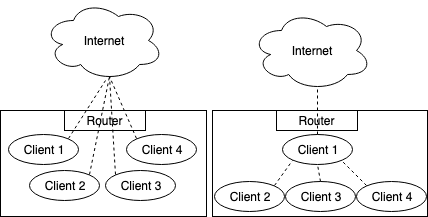
\includegraphics{architecture_shift}
    \caption{Architecture shift: on the left side is the traditional web application architecture where all devices are connected to a web server through the Internet. On the right is the Zeroconf architecture where only one client requires such a connection and becomes a server to all other clients in the network.}
    \label{fig:architecture_shift}
\end{figure}

Evidently, this pattern of communication has one major problem: it has a single point of failure, namely the client acting as a local server. 
Solving this problem was our motivation behind Successorships; whenever the currently serving client failed, a new client in the network was elected as the new server and connectivity in the network was re-established automatically.
Successorship thus provided a framework to build fault-tolerant Zeroconf web applications with an easy-to-use JavaScript API.
However, our decision to built it on Mozilla FlyWeb proved to be a major limitation.
Not only did we limit usage of our library to one specific browser vendor; we found out during the course of the project that Mozilla had already deprecated FlyWeb in favor of other priorities.
To make things worse, FlyWeb had a dependency to a Firefox core component (the module responsible for launching a web server within the browser) that was only shipped in a range of versions of the developer edition of Firefox.
In addition to this platform dependency that would, in essence, prevent our framework to be used in practice, the implementation of the Zeroconf protols in FlyWeb was incredibly slow.
According to our evaluation, recovery from failure of the currently serving client took more than 30 seconds in many cases.
With a continuously growing 'Limitations and Future Work' section, we were finally struck by the discovery of an unresolved issue in FlyWeb that made our framework only work on MacOS.
Despite our thoughtful and eager motivations, we had built a tool that nobody would ever use in practice.
Hence the call to get rid of this dependency entirely and provide our own layer below  Successorships.
